\documentclass[10pt]{article}
\usepackage[margin=0.72in]{geometry}
\usepackage[T1]{fontenc}
\usepackage{lmodern}
\usepackage{amsmath,amssymb}
\usepackage{booktabs,longtable,array}
\usepackage{xcolor}
\usepackage{listings}
\usepackage{tikz}
\usetikzlibrary{arrows.meta,positioning,fit}
\usepackage[hidelinks]{hyperref}

\definecolor{neblue}{HTML}{155E75}
\definecolor{negreen}{HTML}{166534}
\definecolor{nered}{HTML}{991B1B}
\definecolor{negray}{HTML}{F3F4F6}
\lstset{basicstyle=\ttfamily\small,breaklines=true,columns=fullflexible,
  keepspaces=true,showstringspaces=false,frame=single,backgroundcolor=\color{negray}}
\setlength{\parindent}{0pt}
\setlength{\parskip}{5pt}
\setlength{\emergencystretch}{3em}

\title{NeuraEdge Universal\\A Beginner-to-RTL Explanation of the Neuromorphic Transformer Accelerator}
\author{Generated from the implemented RTL, Python runtime, tests, and Vivado flow}
\date{\today}

\begin{document}
\maketitle
\tableofcontents
\clearpage

\section{What the machine is}

NeuraEdge Universal is a programmable arithmetic accelerator for the
\texttt{xc7z020clg400-1} FPGA on a PYNQ-Z2 board. It is not wired to one image
size or one classifier. Software describes work using 128-bit commands, and the
same physical engines can execute matrix multiplication, convolution lowered to
matrix multiplication, binary and ternary spiking arithmetic, residual/vector
operations, integer normalization, LIF neuron updates, lookup-table functions,
and fixed-point SGD with momentum.

For the reproduced CIFAR-10 workload, the source four-timestep Spikingformer
checkpoint classifies 9,555 of 10,000 official test images correctly
(95.55\%). The exported integer-coefficient arithmetic classifies 9,542 images
correctly (95.42\%). The difference is 13 images, or 0.13 percentage points.
These numbers are complete software test-set evaluations. RTL operator tests,
archive-integrity tests, command tests, and routed Vivado reports form separate
evidence and are described later rather than being mixed into the accuracy
number.

\section{Electronics and FPGA concepts from zero}

\subsection{A bit is a voltage range}

Digital logic calls a low voltage ``0'' and a high voltage ``1''. A wire in
SystemVerilog describes a physical connection that will carry one of those
levels after synthesis. A bus such as \texttt{logic [63:0] data} is 64 parallel
wires. It can represent an unsigned integer, a signed two's-complement integer,
eight bytes, or control fields; the surrounding logic determines the meaning.

\subsection{Combinational logic and registers}

Combinational logic is made from lookup tables, carry chains, and dedicated
arithmetic blocks. Its output changes after its input changes. A register is a
bank of flip-flops that copies its input only at a clock edge and remembers the
copied value between edges. The accelerator period is 5 ns, so its target
frequency is

\[
  f = \frac{1}{5\times10^{-9}} = 200\ \text{MHz}.
\]

The complete board design also has an 8 ns (125 MHz) DMA/DDR clock and a 10 ns
(100 MHz) control clock. Separate clocks are like workers stepping to different
metronomes: a multibit value cannot simply be sampled between them. AMD AXI
clock converters therefore use handshake synchronizers and asynchronous FIFOs
to transfer complete transactions without mixing bits from different cycles.

An \texttt{always\_comb} block describes combinational gates. An
\texttt{always\_ff @(posedge clk)} block describes registers updated at the
rising edge. The nonblocking operator \texttt{<=} means all right-hand sides
are sampled from the old cycle and all left-hand registers update together.
This is why the order of nearby nonblocking assignments does not turn them into
sequential software statements.

\subsection{Finite-state machines}

A finite-state machine stores a small state code in registers. Combinational
decode logic selects what happens in each named state. For example, the
descriptor sequencer moves through \texttt{HEADER}, \texttt{COMMAND\_LOW},
\texttt{COMMAND\_HIGH}, \texttt{SUBMIT}, \texttt{PAYLOAD}, and \texttt{WAIT}.
Each transition consumes at least one clock edge, so the waveform exposes the
exact protocol progress.

\subsection{Valid and ready}

AXI-Stream uses a two-sided handshake. The producer raises \texttt{TVALID}
when its data is meaningful. The consumer raises \texttt{TREADY} when it has
space. A transfer occurs only on a rising clock edge where both are 1:

\[
  \text{transfer} = \text{TVALID}\land\text{TREADY}.
\]

If \texttt{TVALID}=1 and \texttt{TREADY}=0, the producer must hold data and
\texttt{TLAST} stable. This is backpressure. The testbenches deliberately stall
ready to prove results are neither lost nor duplicated.

\section{Board-level system}

The Zynq-7020 contains a processing system (PS) and programmable logic (PL) on
one chip. The PS is the dual-core ARM processor running PYNQ/Linux and Python.
The PL is the FPGA fabric containing NeuraEdge. External DDR is connected to the
PS and stores the complete model and large tensors. AXI DMA moves contiguous
buffers between DDR and the accelerator without the ARM copying each word.

\begin{center}
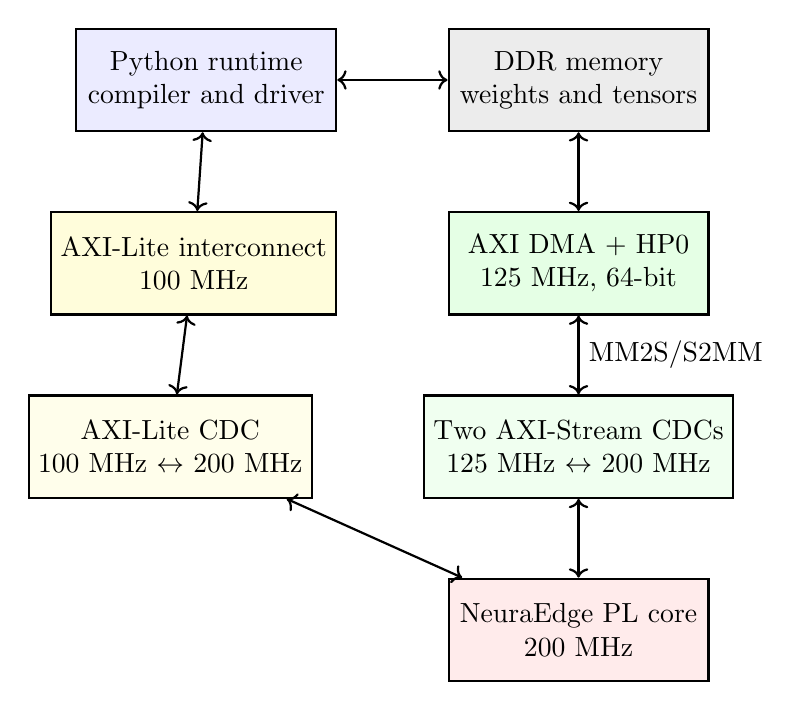
\begin{tikzpicture}[
  block/.style={draw,thick,minimum width=33mm,minimum height=13mm,align=center},
  arrow/.style={-{Latex[length=2.2mm]},thick},node distance=10mm and 14mm]
  \node[block,fill=blue!8] (python) {Python runtime\\compiler and driver};
  \node[block,fill=gray!15,right=of python] (ddr) {DDR memory\\weights and tensors};
  \node[block,fill=green!10,below=of ddr] (dma) {AXI DMA + HP0\\125 MHz, 64-bit};
  \node[block,fill=yellow!14,left=of dma] (lite) {AXI-Lite interconnect\\100 MHz};
  \node[block,fill=green!6,below=of dma] (streamcdc) {Two AXI-Stream CDCs\\125 MHz $\leftrightarrow$ 200 MHz};
  \node[block,fill=yellow!8,left=of streamcdc] (controlcdc) {AXI-Lite CDC\\100 MHz $\leftrightarrow$ 200 MHz};
  \node[block,fill=red!8,below=of streamcdc] (accel) {NeuraEdge PL core\\200 MHz};
  \draw[arrow,<->] (python) -- (ddr);
  \draw[arrow,<->] (ddr) -- (dma);
  \draw[arrow,<->] (dma) -- node[right]{MM2S/S2MM} (streamcdc);
  \draw[arrow,<->] (streamcdc) -- (accel);
  \draw[arrow,<->] (python) -- (lite);
  \draw[arrow,<->] (lite) -- (controlcdc);
  \draw[arrow,<->] (controlcdc) -- (accel);
\end{tikzpicture}
\end{center}

There are three reset controllers, one per domain. Reset assertion brings each
island to a known state; deassertion is synchronized to that island's own
clock. The accelerator never samples a raw 100 or 125 MHz bus. The two stream
clock converters carry \texttt{TDATA}, \texttt{TKEEP}, \texttt{TLAST}, and their
valid/ready state as coherent transactions.

The full Vivado block design uses a 26-bit AXI DMA length field. One legal DMA
packet can therefore contain at most

\[
  2^{26}-1=67{,}108{,}863\ \text{bytes}.
\]

The software driver checks that limit. A larger descriptor program is split
only between records, never through a command header or payload. The PL retains
its model/neuron state between those packets.

\subsection{What Vivado physically implemented}

Vivado 2026.1 routed the complete block design, generated the BIT/HWH/XSA, and
reported zero routing errors. This is the final board result, not the earlier
out-of-context estimate:

\begin{center}
\begin{tabular}{lr}
\toprule
Measured routed quantity & Value\\
\midrule
Worst setup slack / total setup violation & $+0.005$ ns / $0.000$ ns\\
Worst hold slack / total hold violation & $+0.050$ ns / $0.000$ ns\\
Used LUTs / flip-flops & 45,245 / 51,077\\
DSP48E1 / RAMB36 / RAMB18 & 110 / 33 / 8\\
Fully routed nets / routing errors & 74,557 / 0\\
Vectorless total / dynamic estimate & 2.152 W / 1.993 W\\
SAIF total / dynamic estimate & 1.937 W / 1.785 W\\
SAIF full-design net match / confidence & 9,164 of 123,250 / Medium\\
\bottomrule
\end{tabular}
\end{center}

The SAIF estimate attributes 0.472 W dynamic power to the accelerator
hierarchy. Untouched memories produce explicit X-state warnings, so the 93\%
unmatched portion is filled probabilistically by Vivado. These values are
useful implemented-design estimates; they are not relabeled as readings from a
physical board supply rail.

\section{Descriptor programs}

Issuing one AXI-Lite transaction per tile would make the ARM part of every
inner loop. Descriptor mode instead sends a complete program through DMA. Each
record contains the following 64-bit beats:

\begin{longtable}{>{\ttfamily}p{0.18\linewidth}p{0.76\linewidth}}
\toprule
Beat & Exact contents and purpose\\
\midrule
\endhead
header & Bits 31:0 are payload beat count; bits 62:32 are result beat count;
bit 63 marks the final record of this DMA program.\\
command low & Command bits 63:0.\\
command high & Command bits 127:64. If the command has no payload and this is
the final record, input TLAST is asserted here.\\
payload & Exactly the declared number of 64-bit input beats. The sequencer
regenerates the per-command TLAST expected by the selected core engine.\\
\bottomrule
\end{longtable}

The sequencer has a one-beat elastic output register. It can pop the old beat
and capture a new core beat in the same cycle, sustaining one result per cycle
under no backpressure. Declared output counters are deliberately kept out of
the core-ready path. An extra core result is accepted, discarded locally, and
reported as a program error; it cannot deadlock the core or leak into DDR.

\section{Command-driven universal core}

\texttt{neuraedge\_universal\_core.sv} decodes the opcode and connects the
shared input/output streams to exactly one engine. The important engine classes
are:

\begin{longtable}{p{0.25\linewidth}p{0.69\linewidth}}
\toprule
Engine & Physical responsibility\\
\midrule
\endhead
Buffered tensor core & Stores activation/weight tiles, compacts sparse K
positions, schedules dense/binary/ternary work, and streams 32-bit results.\\
Vector ALU & Residual add, maximum, comparisons, ReLU, spike conversion, signed
rounding, saturation, and accumulator requantization on eight lanes.\\
Alpha-XNOR & Spiking self-attention score using matching-one and matching-zero
events.\\
LayerNorm & Integer mean, variance, integer square root, division, learned
gamma/beta, and signed output saturation.\\
Log softmax & Integer power-of-two probability approximation and normalization.\\
LIF bank & 32 persistent membrane states with leak, threshold, reset, and
64-bit spike telemetry.\\
Activation LUT & Eight-lane programmable lookup table for nonlinear functions.\\
SGD optimizer & Eight-lane signed parameter update with momentum, saturation,
and update telemetry.\\
\bottomrule
\end{longtable}

Only the selected engine sees command-valid. Input ready comes from that engine,
and the output arbiter returns only that engine's valid/data/last. A busy engine
must complete before another command is accepted. This simple ownership rule
prevents two engines from driving the same stream simultaneously.

\section{Dense tensor arithmetic}

\subsection{Matrix multiplication}

For matrices $A\in\mathbb{Z}^{M\times K}$ and
$B\in\mathbb{Z}^{K\times N}$, the output is

\[
  C_{m,n}=\sum_{k=0}^{K-1} A_{m,k}B_{k,n}.
\]

The physical tile computes eight output rows and sixteen output columns. It has
64 DSP48E1 blocks, each producing two exact byte products, so 128 byte MAC
lanes are available per cycle. The arithmetic peak at 200 MHz is

\[
  128\times200\times10^6=25.6\ \text{GMAC/s}.
\]

Counting multiply and add as separate operations gives 51.2 GOPS. This is a
peak issue rate, not an application throughput claim: loading, boundaries,
sparsity, vector operations, and DDR can reduce sustained throughput.

\subsection{Two dataflows}

Outer mode broadcasts one K-position activation per row and reuses sixteen
weights across the columns. It is useful for ordinary matrix tiles with several
rows. Dot8 mode feeds eight adjacent K positions into each column and reduces
them, keeping the same DSPs useful when the output has only one row. The
compiler estimates byte traffic for legal schedules and chooses a mode rather
than fixing one traversal for every layer.

\subsection{Exact asymmetric quantization}

An unsigned byte $A$ represents real zero at activation zero point $Z_a$; an
unsigned byte $B$ represents real zero at weight zero point $Z_b$. Direct
centered arithmetic is

\[
  \sum_k(A_k-Z_a)(B_k-Z_b)+\text{bias}.
\]

Expanding the product lets hardware use unsigned DSP products plus row and
column corrections:

\[
  \underbrace{\sum_k A_kB_k}_{\text{raw}}
  -Z_b\underbrace{\sum_k A_k}_{R_a}
  -Z_a\underbrace{\sum_k B_k}_{C_b}
  +KZ_aZ_b+\text{bias}.
\]

The Python golden test evaluates both equations on randomized shapes and zero
points. Equality is exact integer equality; no tolerance hides a mismatch.

\subsection{Two byte products in one DSP}

The packed weight is

\[
  P=B_{lo}+(B_{hi}\ll17).
\]

Multiplying $P$ by activation $A$ places $A B_{lo}$ in bits 15:0 and
$A B_{hi}$ in bits 32:17. Bit 16 is a guard because
$255\times255=65025<2^{16}$. The high packed bit can make the DSP operand appear
signed, so the RTL adds an exact correction through the DSP C input. Vivado's
synthesis log confirms the intended $C+A\times B$ DSP mode, and the testbench
exhaustively checks 131,072 packed input combinations.

\section{Event-driven arithmetic}

Binary weighted mode implements

\[
  y_n=\sum_k s_k w_{k,n},\qquad s_k\in\{0,1\}.
\]

When $s_k=0$, no weight is added. Ternary mode accepts
$t_k\in\{-1,0,+1\}$ and conditionally subtracts, skips, or adds the weight.
The activation loader detects K positions that are zero for every active row
and stores only their surviving indices. Compute then iterates over the compact
list, so an all-zero reduction position removes a cycle instead of merely
presenting zero to a multiplier.

Two hardware counters separate ordinary dense MACs from event-driven weight
adds. They are per-command exact counts, accumulated into wider wrapper
telemetry. This makes activity visible in waveforms and software snapshots.

\section{LIF neurons}

A leaky-integrate-and-fire neuron retains membrane $u[t]$ between timesteps.
The implemented fixed-point order is:

\begin{align*}
  u_{leak}[t] &= \operatorname{roundShift}(u[t-1]\,\lambda),\\
  u_{int}[t] &= u_{leak}[t]+I[t],\\
  s[t] &= [u_{int}[t]\geq\theta],\\
  u[t] &= \begin{cases}u_{reset},&s[t]=1\\u_{int}[t],&s[t]=0.\end{cases}
\end{align*}

$I[t]$ is input current, $\lambda$ is leak, $\theta$ is threshold, and square
brackets produce 1 when the condition is true. The bank stores 32 membranes.
Software chunks a larger logical tensor into banks and executes all timesteps
for one chunk before reusing the physical lanes. Clearing membrane state is
separate from clearing lifetime spike counters, so image boundaries do not
erase telemetry accidentally.

\section{Spiking attention and transformer operations}

Alpha-XNOR compares binary query and key spikes. A matching one contributes
256 in Q8 units; a matching zero contributes programmable $\alpha_{Q8}$:

\[
  score=256N_{11}+\alpha_{Q8}N_{00}.
\]

The ordinary binary QK path used by the exported checkpoint is also supported:
conditional additions form the attention score, a threshold LIF produces an
attention event, unsigned AV aggregation accumulates values, and a vector
requantization applies the exact 0.125 scale. Dense QK, integer LayerNorm,
power-of-two softmax, residual add, and MLP projections remain available for
standard/hybrid transformer graphs.

\section{Exact exported Spikingformer graph}

The executable runtime follows this checkpoint's actual forward function:

\begin{enumerate}
  \item Normalize one $3\times32\times32$ CIFAR-10 image.
  \item Execute five folded tokenizer convolutions. The first projection is
  computed once and broadcast across four timesteps, matching source code.
  \item Apply LIF after each tokenizer stage and binary max-pool at the two
  spatial reduction points, ending at 384 channels and $4\times4$ positions.
  \item For each of four transformer blocks, compute Q, K, and V, reshape into
  12 heads, run spiking QK and AV, apply the output projection, and add the
  attention residual.
  \item Execute the $384\rightarrow1536\rightarrow384$ spiking MLP and add its
  residual.
  \item Average over four timesteps and 16 spatial positions, then execute the
  signed INT8 $384\rightarrow10$ classifier and argmax.
\end{enumerate}

The source checkpoint's forward function does not call LayerNorm, so the
runtime does not insert one. Operator support and model use are different
facts: the accelerator supports LayerNorm for other transformer graphs, while
this exact model does not request it.

The generated manifest totals 3,732,164,352 model MAC equivalents, 104,256 tile
commands, 243,330,192 raw tile-input bytes, and 52,297,808 result values. These
counts come from real exported shapes and the compiler schedule.

\section{Parameter archive and corruption checks}

The hardware archive is 9,385,704 bytes and has SHA-256 digest
\texttt{b02c5df5\allowbreak{}19eaecff\allowbreak{}b228f4c8\allowbreak{}be21babd\allowbreak{}
d0c01761\allowbreak{}f26210bb\allowbreak{}8dfcca33\allowbreak{}18ed0d381}.
It contains 118 64-byte-aligned sections representing 29 folded projections
and the classifier. The loader verifies the whole-file size and digest,
section order and uniqueness, non-overlap and bounds, dtype/shape byte counts,
each section digest, and every projection reference. Returned NumPy views are
read-only so execution cannot silently modify trained parameters.

\section{Host compiler and memory behavior}

The compiler validates dimensions before allocating DMA buffers. Convolution
is lowered to rows of receptive-field values and then tiled as GEMM. Group,
stride, padding, dilation, depthwise binary, and depthwise ternary cases have
directed tests. The compact stream representation stores each 64-bit beat once
in a standard-library integer array instead of expanding millions of Python
objects.

For the real block-3 shape $1024\times1728\times384$, the recorded benchmark
produces 6,168 instructions, 43,130,880 payload bytes, 148,032 descriptor bytes,
43,278,912 total input bytes, and 3,145,728 output bytes. Vectorized packing
took 0.334 s in the recorded run; the former scalar implementation took
95.601 s for the same case.

\section{Full-backbone on-device training flow}

The training entry point uses the same exported 29 projections and classifier
as inference. A minibatch follows this exact order:

\begin{enumerate}
  \item Read a hashed official CIFAR-10 shard, apply a deterministic reflected
  crop and horizontal flip, and normalize the resulting RGB samples.
  \item Run the complete quantized forward graph while retaining projection
  inputs, pre-reset LIF membranes, spikes, pool inputs, attention operands, and
  residual branch values needed by the reverse pass.
  \item Evaluate the ten-way power-of-two softmax in programmable logic. The
  vector ALU forms the Q15 batch-mean classifier derivative
  $p-\operatorname{onehot}(y)$.
  \item Traverse the graph in reverse: classifier, four transformer blocks,
  tokenizer, and finally the input image. Every converging residual branch is
  added explicitly and every parameter name must appear exactly once.
  \item Convert each block-floating parameter gradient to Q15, clamp it in the
  vector fabric, update its signed master and momentum tensors in the optimizer
  lanes, and redeploy the rounded/clamped inference tensor.
  \item Atomically checkpoint every master tensor, every momentum tensor,
  optimizer step, epoch, next minibatch index, graph identity, and numeric
  format before a pause or according to the configured checkpoint interval.
\end{enumerate}

The complete 9.3 MB parameter state cannot fit in the Zynq-7020's roughly
630 KiB of block RAM. Master tensors and saved activations therefore reside in
board DDR, while matrix backward, vector gradient algebra, nonlinear
derivatives, and parameter updates execute in programmable logic. DMA moves
bounded tiles; it does not replace an FPGA arithmetic result with a NumPy
calculation.

The generated coverage manifest derives its counts from the exported graph. It
contains 43 of 43 execution operators, 30 learned affine groups, eight dynamic
attention matrix products, 32 LIF sites, two max-pool sites, and eight residual
fan-outs, with zero uncovered operators. One full sample schedules 14,742,724
backward partial tiles and 7,474,847,252 signed backward multiplications across
9,295,978 deployed trainable parameter elements.

\subsection{Exact matrix and convolution derivatives}

For one affine layer

\[
  Y=XW+b,
\]

the reverse equations implemented by the training compiler and signed backward
array are

\[
  dX=dY W^{T},\qquad dW=X^{T}dY,\qquad db=\sum_m dY_m.
\]

The compiler appends a column of ones to $X$ and a bias row to $W$, so the same
verified matrix engine produces $dW$ and $db$ without a host-side reduction.
Arbitrary dimensions are partitioned into at-most $8\times8$ external tiles.
For $dX$, one row/input tile remains in the 47-bit accumulator while every
output-feature tile is traversed. For $dW$, one input/output tile remains while
every sample-row tile is traversed. Intermediate commands suppress output; only
the last reduction chunk performs one signed round and streams the final tile.

Inside \texttt{neuraedge\_linear\_backward8.sv}, a physical $4\times4$ signed
DSP array visits two result-column groups and, when needed, two reduction
groups. Sixteen registered $16\times16$ products become two 33-bit pair sums,
one 34-bit four-product sum, and a mathematically sufficient 35-bit local sum.
That sum is sign-extended only when added to the retained 47-bit accumulator.
Magnitude, rounding bias, shift, sign restoration, saturation, and result
storage occupy separate states so no combinational carry chain spans all those
operations at 200 MHz.

Convolution backward uses the same equations after exact signed
\texttt{im2col}. Group, stride, padding, dilation, and kernel coordinates are
retained in the compiled plan. The returned patch gradient is scattered back
with saturating overlap addition; grouped and depthwise shapes never mix
channels from different groups.

\subsection{LIF, pooling, attention, and residual derivatives}

Hard thresholding has zero derivative almost everywhere, so training uses the
SpikingJelly sigmoid surrogate with $\alpha=4$. A generated 256-entry Q15 table
stores

\[
  \sigma'(x)=\alpha\sigma(\alpha x)(1-\sigma(\alpha x)).
\]

The address is the saturated, rounded pre-reset membrane distance from the
threshold. Reverse-time BPTT walks the four cached timesteps from 3 to 0. With
detached hard reset, the temporal membrane path is cleared where the forward
step spiked; leak, surrogate multiplication, and input scaling are Q15 vector
operations with explicit signed saturation.

Max-pool backward reproduces PyTorch's first-maximum tie rule, then uses fabric
maximum/comparison and scatter-add operations to return gradients to the chosen
input coordinates. Dynamic QK and AV products use the same two matrix-backward
passes as learned projections. Attention's exact factor 0.125 is a power-of-two
gradient shift. Residual addition copies the incoming derivative to both
parents; derivatives from branches that meet later are combined by the
saturating vector adder.

\section{On-chip parameter update engine}

The SGD engine accepts current signed weights $w$, signed gradients $g$, and
momentum state $v$. Its fixed-point form is

\begin{align*}
  v' &= \operatorname{roundShift}(\mu v)+g,\\
  d  &= \operatorname{sat}\left(v'+\operatorname{roundShift}(\lambda w)\right),\\
  w' &= \operatorname{sat}\left(w-\operatorname{roundShift}(\eta d)\right).
\end{align*}

$\mu$ is momentum, $\eta$ is learning rate, and $\lambda$ is weight decay.
The retained velocity $v'$ contains the loss gradient and momentum only;
decay enters the temporary direction $d$ and therefore cannot accumulate in
the momentum state. This is the SGDW decoupling defined by Loshchilov and
Hutter. Rounding is symmetric for positive and negative values, and saturation
clamps rather than wrapping at the signed limits. The update loop processes
eight lanes, writes both new weight and velocity state, and increments an exact
update counter. The same tensor engine can execute matrix products needed for
gradient formation; the optimizer is the fabric-resident primitive that
applies those gradients.

\section{Verification evidence}

\begin{longtable}{p{0.31\linewidth}p{0.63\linewidth}}
\toprule
Gate & Evidence and what it proves\\
\midrule
\endhead
Python unit suite & 93 protocol, compiler, quantized algebra,
archive integrity, full-model graph pieces, DMA ordering, and build contracts.\\
Verilator strict lint & All synthesizable RTL parses with warnings treated as
reviewed failures by the project script.\\
Icarus RTL suite & Four-state simulation of 15 testbenches, including reset,
backpressure, boundaries, exhaustive packed MACs, descriptor overrun, and
independent fixture comparison.\\
Full CIFAR-10 software evaluation & 95.55\% checkpoint and 95.42\% exported
integer arithmetic over exactly 10,000 official test images.\\
Vivado OOC implementation & Accelerator-only iteration closes 200 MHz with
$+0.031$ ns setup slack and zero route/DRC errors. Its top-port hold result is
explicitly labeled as OOC context because no board part-pin locations exist.\\
Full PYNQ implementation & Processing system, three clock/reset domains,
AXI-Lite and stream CDC, DMA, HP0 DDR path, and accelerator route with
$+0.005$ ns setup and $+0.050$ ns hold slack; BIT, HWH, XSA, and DCP are hashed.\\
DRC and CDC audit & Zero DRC errors; 122 named DRC warnings and three AMD
interconnect methodology warnings are retained. CDC warnings resolve to AMD
XPM asynchronous FIFO internals and their declared timing exceptions.\\
SAIF power flow & Two XSim activity files are relocated to the exact full-design
accelerator hierarchy, matching 9,164 nets before the medium-confidence
1.937 W total estimate.\\
Physical-board measurement & Supply-rail energy and wall-clock throughput must
come from a connected board and are kept distinct from Vivado estimates.\\
\bottomrule
\end{longtable}

\section{Where every line is explained}

The companion file \texttt{neuraedge\_line\_by\_line\_source\_reference.tex}
contains every RTL, Python, PowerShell, Tcl, and test source file. It includes
the complete numbered source and a context-aware annotation for every nonblank
line. Its JSON manifest records SHA-256 for every included source, preventing a
PDF from being mistaken for documentation of a later code revision.

The 55-page
\texttt{outputs/deep\_debug\_final/neuraedge\_deep\_debug\_report.pdf}
contains 49 generated evidence plots, all 15 XSim waveform views, artifact
hashes, full timing/resource/DRC/CDC/power plots, and the native Vivado
\texttt{system.bd} export.

The final line-by-line PDF contains 99 source files, 28,915 physical source
lines, and an explanation for all 26,565 nonblank lines. Its generated length
is 3,277 pages.

\section{Primary research and vendor references}

\begin{sloppypar}
\begin{itemize}
  \item Spikingformer: \url{https://arxiv.org/abs/2304.11954}
  \item FlashAttention IO-aware exact attention: \url{https://arxiv.org/abs/2205.14135}
  \item I-ViT integer-only vision transformer: \url{https://arxiv.org/abs/2207.01405}
  \item FQ-ViT: \url{https://arxiv.org/abs/2111.13824}
  \item Alpha-XNOR spiking attention: \url{https://openaccess.thecvf.com/content/CVPR2025/html/Xiao_Rethinking_Spiking_Self-Attention_Mechanism_Implementing_a-XNOR_Similarity_Calculation_in_Spiking_CVPR_2025_paper.html}
  \item AMD AXI DMA PG021: \url{https://docs.amd.com/r/en-US/pg021_axi_dma/Field-Descriptions}
  \item AMD Vivado power analysis UG907: \url{https://docs.amd.com/r/en-US/ug907-vivado-power-analysis-optimization/Running-Power-Analysis-from-the-Vivado-IDE}
\end{itemize}
\end{sloppypar}

\end{document}
